\chapter{Systembeschreibung und Durchführung}
\label{ch:durchfuehrung}

Dieses Kapitel beschreibt die konkret umgesetzte Systemarchitektur sowie die methodische Durchführung der Implementierung und Validierung des Follow-the-Gap-Stacks im Repository \texttt{ftg\_mxck}. Der Fokus liegt auf dem scan-basierten Hauptpfad, der als primäre Laufzeitarchitektur definiert wurde.

\section{Gesamtarchitektur des Systems}

Die entwickelte Pipeline folgt einer strikt modularen Struktur, die sich in vier logisch getrennte Verarbeitungsebenen gliedert:

\begin{enumerate}
    \item LiDAR-Vorverarbeitung (Perception)
    \item Reaktiver Planerkern (Follow-the-Gap)
    \item Policy-basierte Entscheidungslogik (Planner)
    \item Fahrzeugschnittstelle (Control)
\end{enumerate}

Die resultierende Datenflusskette ist in Abbildung~\ref{fig:system_pipeline} dargestellt.

\begin{figure}[H]
    \centering
    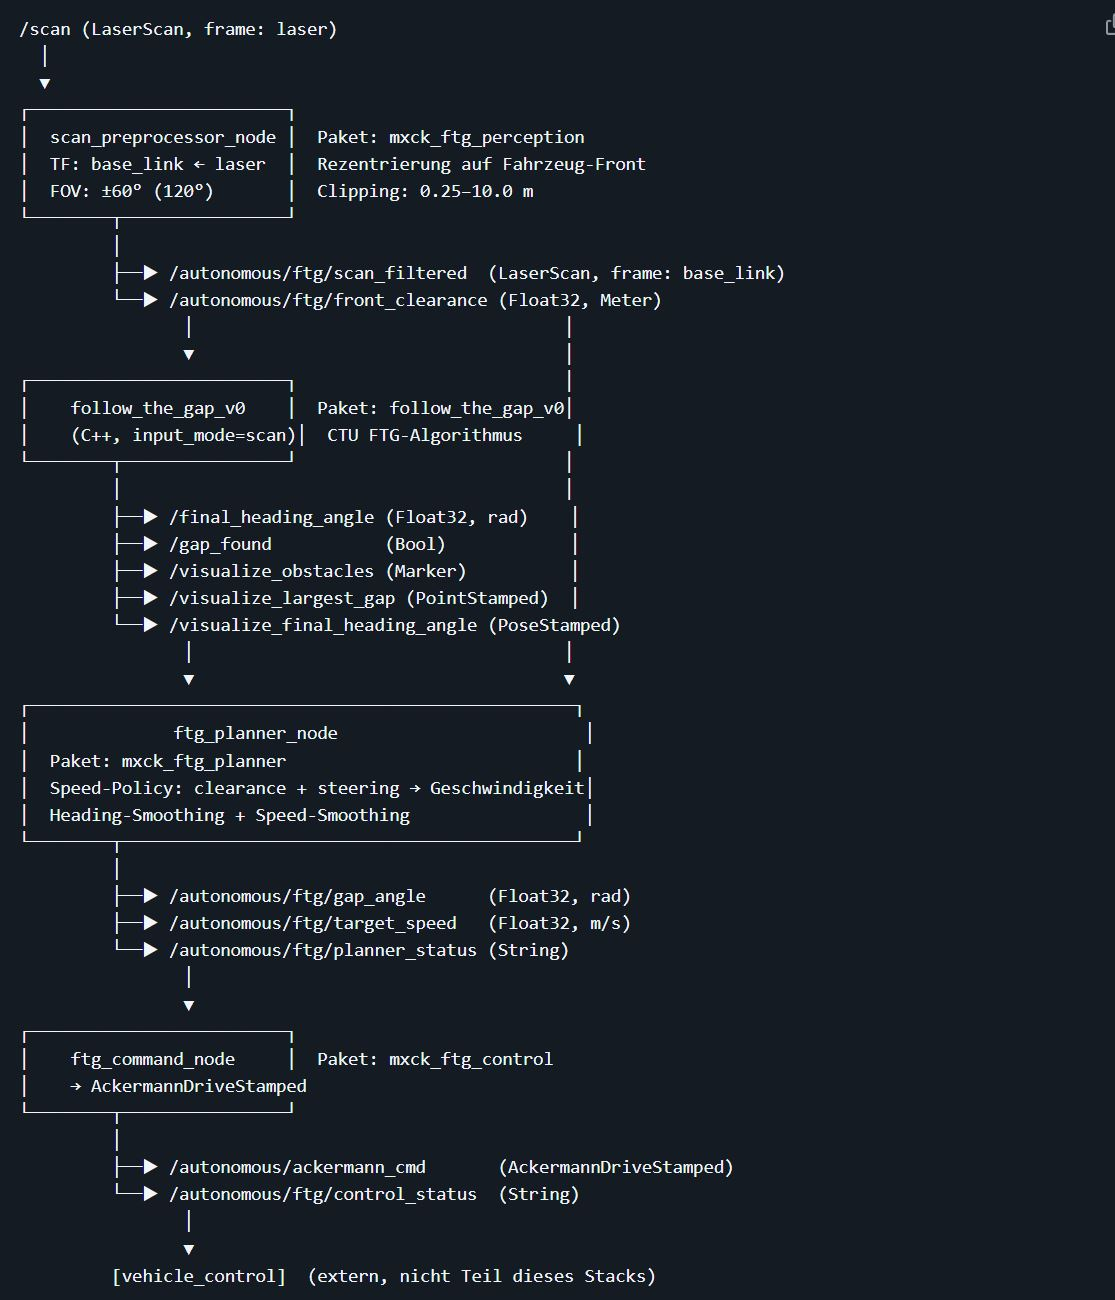
\includegraphics[width=0.85\textwidth]{images/Gesamtarch.JPG}
    \caption{Gesamtarchitektur des scan-basierten FTG-Stacks . Die Pipeline reicht vom Rohscan bis zur Ackermann-Ausgabe und zeigt die klare Trennung zwischen Wahrnehmung, Planung und Steuerung.\cite{mxck_repo}}
    \label{fig:system_pipeline}
\end{figure}

Der vollständige Aufbau sowie alle Konfigurationsdateien sind im Repository \texttt{ftg\_mxck} dokumentiert. Im Rahmen dieser Arbeit wird auf eine vollständige Reproduktion aller Startbefehle verzichtet; stattdessen wird die Architektur konzeptionell beschrieben und auf die implementierten Komponenten verwiesen.

\section{Algorithmische Grundlage}

Der eingesetzte Planungsansatz basiert auf dem Follow-the-Gap-Verfahren nach Sezer und Gokasan~\cite{sezer2012}. Die konkrete Implementierung orientiert sich an der F1TENTH-/CTU-Referenz~\cite{ctu_ftg} und wurde unverändert als C++-Kern in den Stack integriert.

\begin{figure}[H]
    \centering
    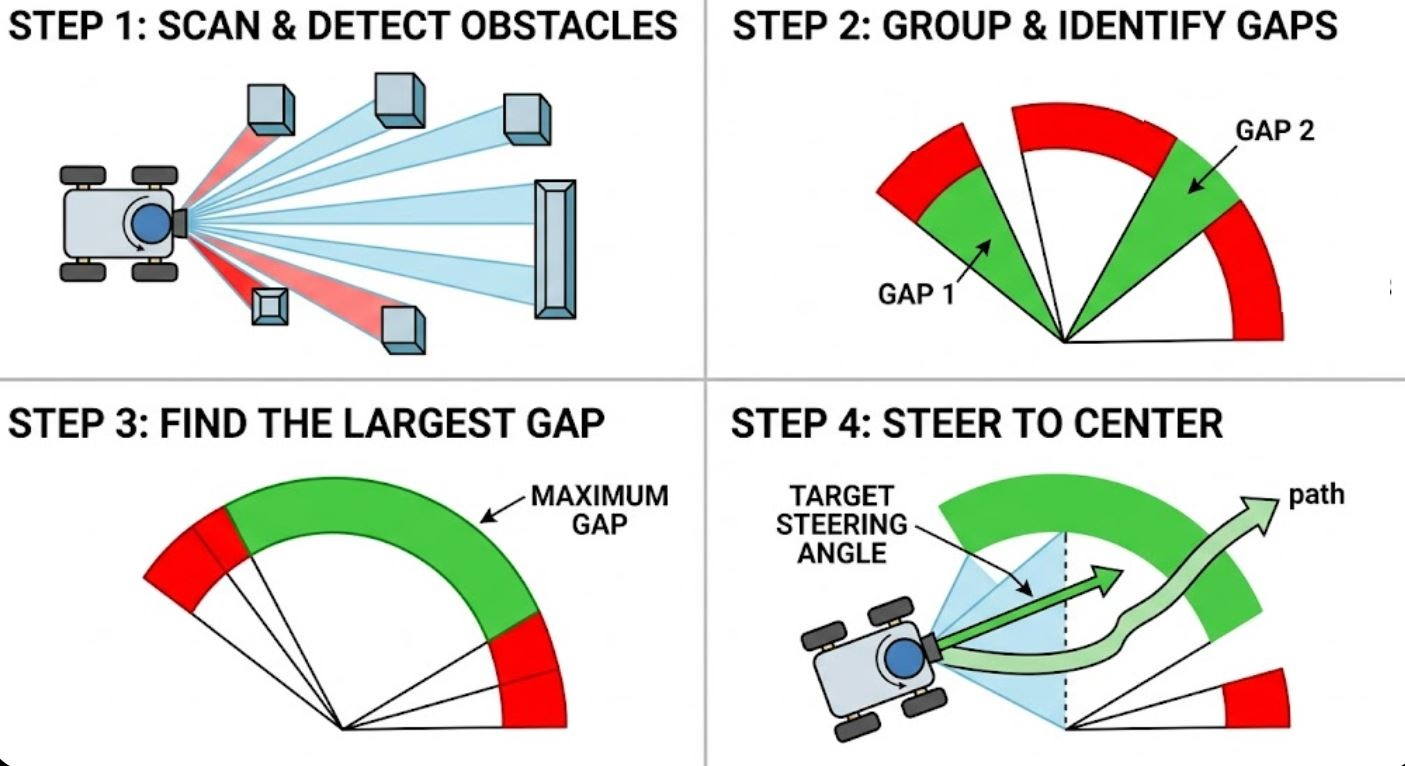
\includegraphics[width=1\textwidth]{images/ftg_algorithm1.JPG}
    \caption{Schematische Darstellung des Follow-the-Gap-Prinzips \cite{ai2026}.}
    \label{fig:ftg_algorithm}
\end{figure}

Die zentrale Idee besteht darin, aus einem eindimensionalen Distanzprofil die größte kollisionsfreie Lücke zu bestimmen und das Fahrzeug entlang deren Mittelpunkt auszurichten. Diese Strategie ermöglicht eine robuste reaktive Navigation ohne globale Karteninformation.

\section{Stufe 1: LiDAR-Vorverarbeitung}

Die Vorverarbeitung transformiert den Rohscan in eine für den FTG-Kern geeignete Repräsentation.

\subsection{Funktionale Aufgaben}

Die implementierte Verarbeitung umfasst:

\begin{itemize}
    \item Transformation des Scans in den Fahrzeugrahmen mittels TF,
    \item Definition eines frontalen Sichtfensters,
    \item Entfernung ungültiger Messwerte,
    \item Glättung des Signals zur Rauschreduktion,
    \item Berechnung des minimalen Frontabstands.
\end{itemize}

Diese Schritte sind notwendig, um die geometrische Konsistenz zwischen Sensor und Fahrzeug sicherzustellen.

\subsection{Node Perception Erklärung}
Bla Bla Bla

\section{Stufe 2: Follow-the-Gap-Kern}

Der Planerkern bildet das algorithmische Zentrum des Systems. Er verarbeitet den vorbereiteten Scan und berechnet daraus einen Richtungswinkel.

\subsection{Verarbeitungsschritte}

Innerhalb des Algorithmus erfolgen:

\begin{enumerate}
    \item Identifikation von Hindernisbereichen,
    \item Bestimmung zusammenhängender freier Bereiche (Gaps),
    \item Auswahl des größten befahrbaren Gaps,
    \item Berechnung eines Zielwinkels innerhalb dieses Gaps.
\end{enumerate}

\subsection{Ausgabegrößen}

Der Algorithmus liefert:

\begin{itemize}
    \item einen kontinuierlichen Heading-Winkel,
    \item ein binäres Signal zur Gap-Erkennung.
\end{itemize}

Diese Ausgabe ist bewusst fahrzeugagnostisch gehalten und enthält keine Informationen über Geschwindigkeit oder Dynamik.

\section{Stufe 3: Planner}

Der Planner interpretiert die algorithmische Ausgabe im Kontext der Fahrzeugdynamik und Sicherheitsanforderungen.

\subsection{Funktionale Rolle}

Im Gegensatz zum FTG-Kern handelt es sich hierbei nicht um einen Planungsalgorithmus im engeren Sinne, sondern um eine Entscheidungslogik, die folgende Aufgaben übernimmt:

\begin{itemize}
    \item Validierung der Eingangsdaten (Freshness),
    \item Begrenzung des Lenkwinkels,
    \item adaptive Geschwindigkeitswahl in Abhängigkeit vom Frontabstand,
    \item Zustandsbewertung des Systems.
\end{itemize}

\subsection{Interpretation der Sensordaten}

Die Geschwindigkeit wird als Funktion des minimalen Abstands gewählt. Dabei gilt:

\begin{itemize}
    \item große Abstände $\rightarrow$ hohe Geschwindigkeit,
    \item kleine Abstände $\rightarrow$ reduzierte Geschwindigkeit,
    \item kritische Abstände $\rightarrow$ Stopp.
\end{itemize}

Diese Policy stellt sicher, dass der reaktive Charakter des FTG-Ansatzes nicht zu unsicheren Fahrzuständen führt.

\section{Stufe 4: Control}

Die letzte Stufe des Systems übernimmt die Transformation der Planner-Ausgabe in fahrzeugspezifische Steuerbefehle.

\subsection{Aufgabe}

Die berechneten Sollwerte werden in ein Ackermann-kompatibles Nachrichtenformat überführt und an die bestehende Fahrzeugsteuerung übergeben.

\subsection{Systemintegration}

Ein wesentliches Designkriterium ist, dass die bestehende Sicherheits- und Steuerlogik des MXCarkit unverändert bleibt. Der entwickelte Stack liefert ausschließlich Sollwerte und greift nicht direkt in die Aktorik ein.

\section{Versuchsdurchführung}

Die Validierung des Systems erfolgte anhand realer Fahrversuche im Innenraum.

\subsection{Versuchsaufbau}

Die Tests wurden in einem strukturierten Korridor durchgeführt, der durch gezielt platzierte Hindernisse definiert wurde.

\begin{figure}[H]
    \centering
    % PLACEHOLDER: Teststrecke 1
    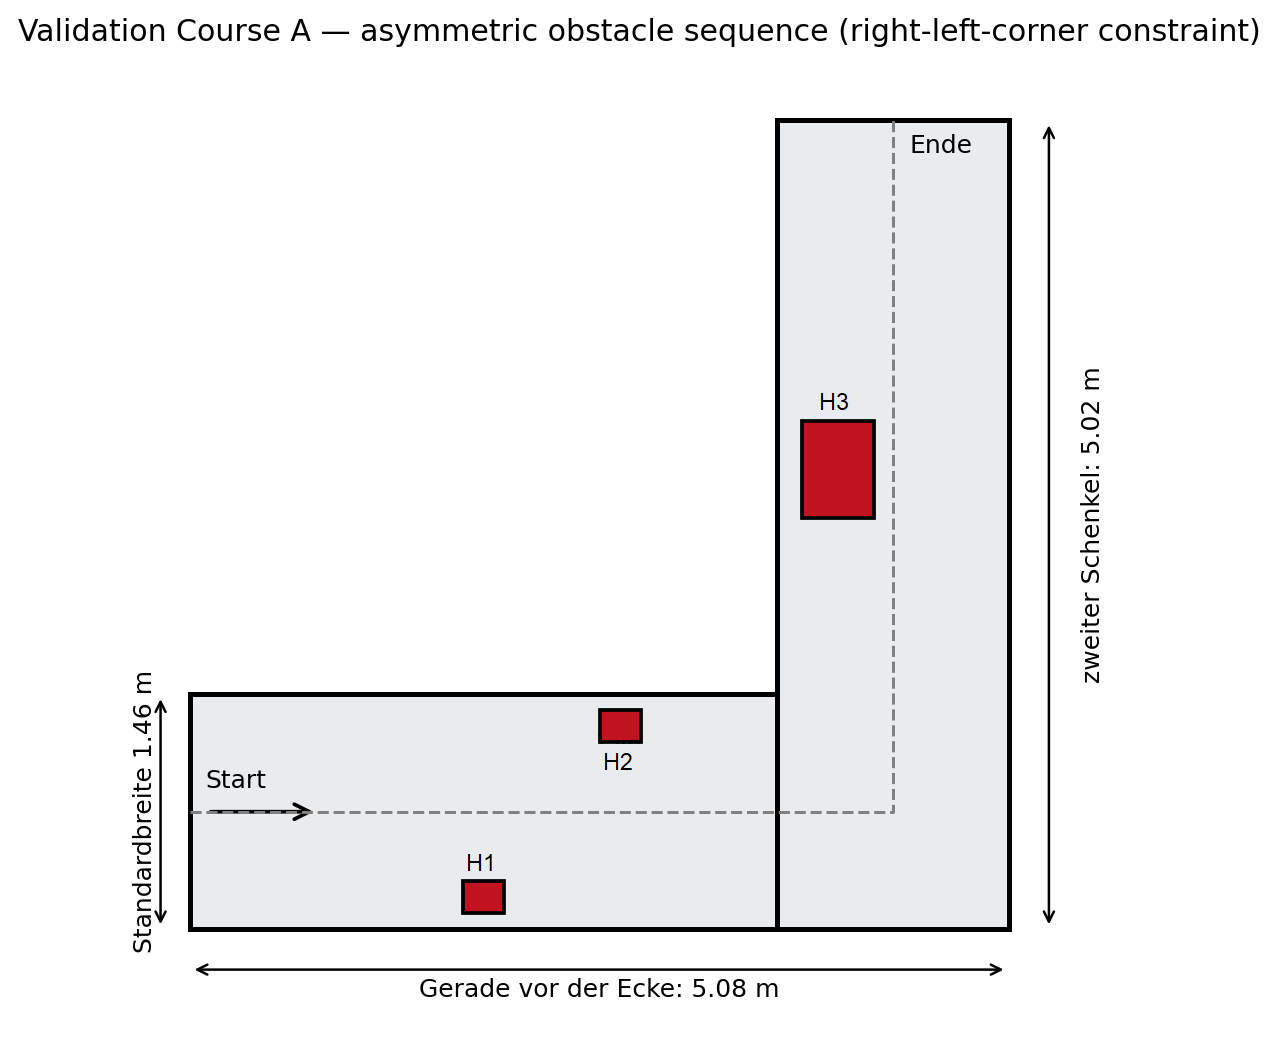
\includegraphics[width=0.75\textwidth]{images/validation_course_A_schematic.png}
    \caption{Versuchsaufbau Aufnahme 1: Korridor mit einem statischen Hindernis.}
    \label{fig:test_track1}
\end{figure}

\begin{figure}[H]
    \centering
    % PLACEHOLDER: Teststrecke 2
    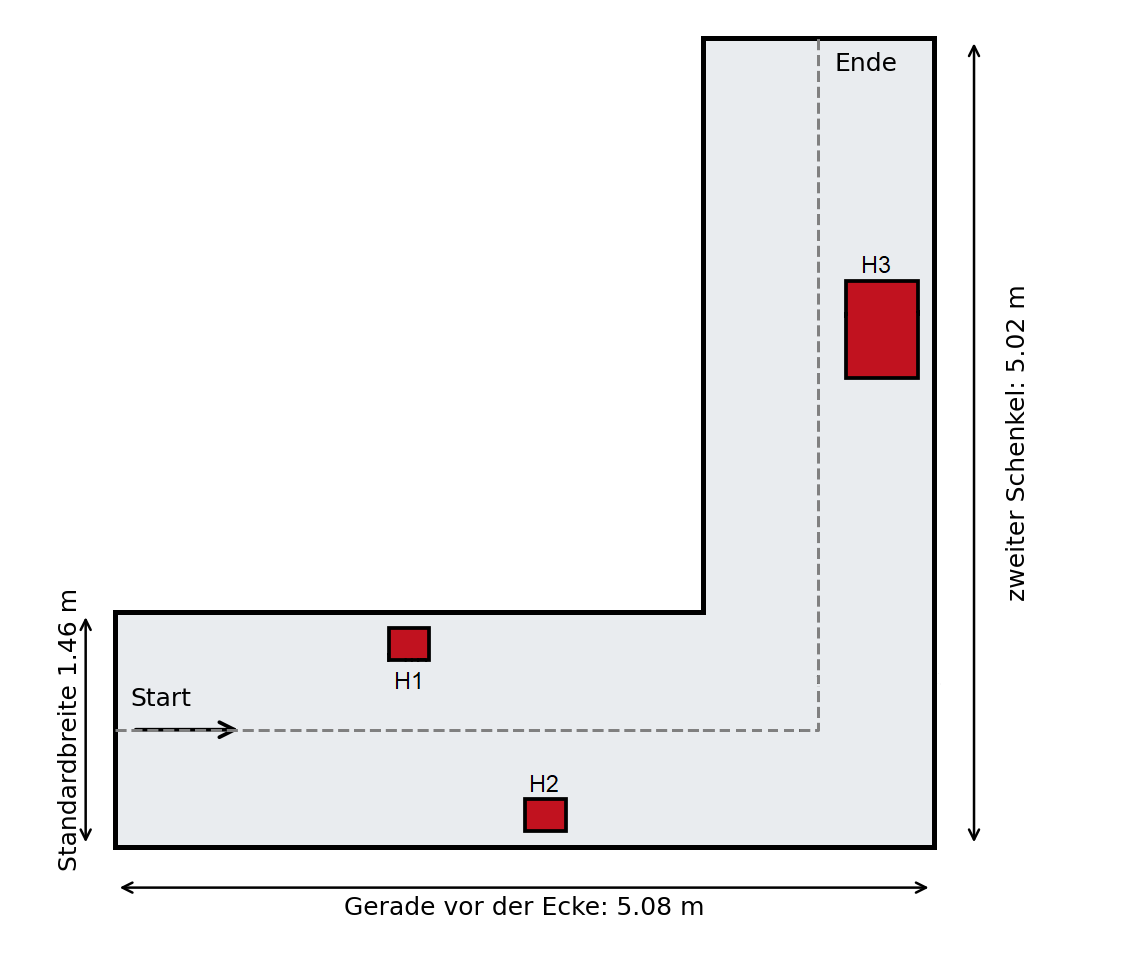
\includegraphics[width=0.75\textwidth]{images/validation_course_B_schematic.png}
    \caption{Versuchsaufbau Aufnahme 2: Mehrere Hindernisse und dynamische Veränderung der Umgebung.}
    \label{fig:test_track2}
\end{figure}
\subsection{Parametrierung des Systems}
\label{sec:parametrierung_system}

Die Validierungsfahrten wurden mit einer fest definierten Konfiguration des FTG-Stacks durchgeführt. 
Die Parametrierung ist für die Bewertung des Systemverhaltens von zentraler Bedeutung, da sie sowohl die 
geometrische Interpretation der Umgebung als auch die resultierende Fahrdynamik direkt beeinflusst. 
Insbesondere wirken sich Sichtfeld, Distanzgrenzen, Geschwindigkeitsgrenzen sowie die Abbremslogik 
unmittelbar auf das Ausweich- und Kurvenverhalten des Fahrzeugs aus.

Tabelle~\ref{tab:ftg_runtime_parameter} fasst die im Validierungsbetrieb verwendeten Laufzeitparameter 
der drei zentralen Softwarestufen Perception, Planner und Control zusammen.

\renewcommand{\arraystretch}{1.2}
\begin{longtable}{p{2.6cm} p{3.0cm} p{1.8cm} p{6.2cm}}
\caption{Verwendete Laufzeitparameter des FTG-Stacks während der Validierungsfahrten.}
\label{tab:ftg_runtime_parameter}\\
\toprule
\textbf{Stufe / Node} & \textbf{Parameter} & \textbf{Wert} & \textbf{Bedeutung und Einfluss auf das Fahrverhalten} \\
\midrule
\endfirsthead

\toprule
\textbf{Stufe / Node} & \textbf{Parameter} & \textbf{Wert} & \textbf{Bedeutung und Einfluss auf das Fahrverhalten} \\
\midrule
\endhead

Perception & \texttt{front\_center\_deg} & 0.0 & Definition der Fahrtrichtung im \texttt{base\_link}-Frame; die physische LiDAR-Montage wird über TF berücksichtigt. \\
Perception & \texttt{front\_fov\_deg} & 180.0 & Breite des für FTG verwendeten Sichtfensters; größere Werte erhöhen die Umgebungsabdeckung, lassen aber seitliche Wände stärker in die Entscheidungsfindung einfließen. \\
Perception & \texttt{clip\_min\_range\_m} & 0.25 & Untere Distanzgrenze; unterdrückt sehr nahe Punkte und mögliche Eigenreflexionen des Fahrzeugs. \\
Perception & \texttt{clip\_max\_range\_m} & 10.0 & Obere Distanzgrenze; begrenzt die Auswertung auf den relevanten Messbereich. \\
Perception & \texttt{enable\_moving\_average} & \texttt{true} & Aktiviert eine Glättung des Distanzsignals zur Reduktion einzelner Ausreißer. \\
Perception & \texttt{moving\_average\_window} & 3 & Fenstergröße der Mittelung; größere Werte erhöhen die Glättung, reduzieren aber die Reaktivität. \\

Planner & \texttt{input\_timeout\_sec} & 0.50 & Maximales Alter der Eingangsdaten; bei Überschreitung wird aus Sicherheitsgründen gestoppt. \\
Planner & \texttt{max\_abs\_gap\_angle\_rad} & 0.45 & Begrenzung des resultierenden Lenkwinkels. \\
Planner & \texttt{cruise\_speed\_mps} & 0.45 & Maximale Sollgeschwindigkeit bei freier Umgebung. \\
Planner & \texttt{min\_speed\_mps} & 0.20 & Untergrenze der Fahrgeschwindigkeit im normalen Betrieb. \\
Planner & \texttt{stop\_speed\_mps} & 0.00 & Sollgeschwindigkeit im Stoppfall. \\
Planner & \texttt{stop\_clearance\_m} & 0.25 & Kritischer Frontabstand, unterhalb dessen das Fahrzeug anhalten soll. \\
Planner & \texttt{caution\_clearance\_m} & 0.50 & Abstand, ab dem wieder die volle Clearance-Freigabe erreicht wird. \\
Planner & \texttt{steering\_slowdown\_start\_rad} & 0.40 & Ab diesem Lenkwinkel wird die Geschwindigkeit schrittweise reduziert. \\
Planner & \texttt{steering\_slowdown\_full\_rad} & 0.70 & Lenkwinkelbereich für maximale Geschwindigkeitsreduktion; bewusst größer als der maximal zulässige Gap-Winkel gewählt, um Corner-Blockaden zu vermeiden. \\
Planner & \texttt{heading\_smoothing\_alpha} & 0.4 & Glättungsfaktor für den Heading-Winkel; reduziert sprunghafte Richtungswechsel zwischen aufeinanderfolgenden Scans. \\
Planner & \texttt{speed\_smoothing\_alpha} & 0.3 & Glättungsfaktor für die Beschleunigungsphase; Bremsvorgänge bleiben davon unberührt und werden direkt umgesetzt. \\

Control & \texttt{input\_timeout\_sec} & 0.50 & Sicherheitsgrenze für veraltete Planner-Daten; bei Überschreitung wird ein Nullkommando ausgegeben. \\
Control & \texttt{angle\_to\_steering\_gain} & -1.00 & Vorzeichen- und Skalierungsfaktor für die Lenkabbildung; negative Werte invertieren die physische Lenkreaktion. \\
Control & \texttt{max\_steering\_angle\_rad} & 0.45 & Hardwarebedingte Begrenzung des Lenkwinkels. \\
Control & \texttt{min\_speed\_mps} & 0.18 & Untere Grenze der ausgegebenen Sollgeschwindigkeit. \\
Control & \texttt{max\_speed\_mps} & 1.80 & Obergrenze der ausgegebenen Sollgeschwindigkeit. \\
\bottomrule
\end{longtable}

Neben den Laufzeitparametern verwendet der C++-Kern \texttt{follow\_the\_gap\_v0} zusätzlich interne,
nicht zur Laufzeit parametrierbare Geometrie- und Gewichtungskonstanten. Diese sind in
Tabelle~\ref{tab:ftg_internal_constants} zusammengefasst, da sie die Passierbarkeit von Lücken und
damit das resultierende Fahrverhalten ebenfalls wesentlich beeinflussen.


\begin{table}[H]
\centering
\caption{Interne FTG-Konstanten des C++-Kerns \texttt{follow\_the\_gap\_v0}.}
\label{tab:ftg_internal_constants}
\begin{tabularx}{\textwidth}{l l X}
\toprule
\textbf{Konstante} & \textbf{Wert} & \textbf{Bedeutung} \\
\midrule
\texttt{kCarRadius} & 0.40 m & Effektiver Sicherheitsradius zur Hindernis-Aufblähung und damit maßgeblich für die als passierbar bewertete Gap-Breite. \\
\texttt{kTurnRadius} & 0.30 m & Modellannahme für die Kurvenfähigkeit des Fahrzeugs. \\
\texttt{kTrackMinWidth} & 0.35 m & Mindestbreite für bestimmte Corner- und Gap-Bewertungen. \\
\texttt{kDistanceToCorner} & 0.22 m & Sicherheitsabstand bei Corner-bezogenem Verhalten. \\
\texttt{kGapWeightCoefficient} & 100.0 & Gewichtung der Gap-Richtung in der Zielrichtungsbestimmung. \\
\texttt{kCornerWeightCoefficient} & 100.0 & Gewichtung corner-spezifischer Anteile in der Zielwahl. \\
\bottomrule
\end{tabularx}
\end{table}

Die tabellarische Zusammenstellung ist für die Reproduzierbarkeit der Ergebnisse essenziell, da bereits
moderate Änderungen einzelner Parameter zu deutlich unterschiedlichem Fahrverhalten führen können. 
Insbesondere das Sichtfeld, die Clearance-Schwellen sowie der effektive Fahrzeugradius beeinflussen, 
ob enge Passagen als befahrbar oder blockiert interpretiert werden.

\subsection{Messmethodik und Datenerfassung}
\label{sec:messmethodik}

Zur experimentellen Bewertung des Systems wurden sämtliche relevanten Systemgrößen während der Fahrt
zeitlich synchron aufgezeichnet und anschließend offline ausgewertet. Die Datenerfassung erfolgte mit
\texttt{rosbag2}, sodass sowohl Rohdaten als auch Zwischen- und Ausgangsgrößen des gesamten FTG-Stacks
reproduzierbar analysiert werden konnten.

Die Auswertung fokussierte sich auf vier zentrale Beobachtungsgrößen:

\begin{itemize}
    \item \textbf{Distanzverlauf:} Charakterisierung der Umgebungssituation über den gefilterten Scan sowie den minimalen Frontabstand,
    \item \textbf{Heading-Winkel:} Bewertung der vom FTG-Kern bestimmten Zielrichtung und deren Weiterverarbeitung im Planner,
    \item \textbf{Geschwindigkeit:} Analyse der Sollgeschwindigkeit des Planners und der tatsächlich ausgegebenen Ackermann-Geschwindigkeit,
    \item \textbf{Gap-Erkennung:} Bewertung, ob und wie stabil freie, befahrbare Lücken detektiert wurden.
\end{itemize}

Die aufgezeichneten Topics deckten sowohl den sensorischen Eingang als auch alle relevanten
Zwischenstufen des Verarbeitungsgraphen ab. Tabelle~\ref{tab:recorded_topics} zeigt die
für die Validierung herangezogenen Nachrichtenströme.

\begin{table}[H]
\centering
\caption{Für die Validierung aufgezeichnete Topics des FTG-Stacks.}
\label{tab:recorded_topics}
\begin{tabular}{p{5.2cm} p{3.2cm} p{6.0cm}}
\toprule
\textbf{Topic} & \textbf{Nachrichtentyp} & \textbf{Funktion in der Auswertung} \\
\midrule
\texttt{/scan} & \texttt{sensor\_msgs/LaserScan} & Rohdaten des LiDARs als Eingangssignal \\
\texttt{/autonomous/ftg/scan\_filtered} & \texttt{sensor\_msgs/LaserScan} & vorverarbeiteter, rezentrierter Scan für FTG \\
\texttt{/autonomous/ftg/front\_clearance} & \texttt{std\_msgs/Float32} & minimaler Frontabstand als Eingangsgröße der Speed-Policy \\
\texttt{/final\_heading\_angle} & \texttt{std\_msgs/Float32} & vom FTG-Kern berechnete Zielrichtung \\
\texttt{/gap\_found} & \texttt{std\_msgs/Bool} & binäre Information über erkannte befahrbare Lücken \\
\texttt{/autonomous/ftg/gap\_angle} & \texttt{std\_msgs/Float32} & begrenzter Planner-Lenkwinkel \\
\texttt{/autonomous/ftg/target\_speed} & \texttt{std\_msgs/Float32} & vom Planner berechnete Sollgeschwindigkeit \\
\texttt{/autonomous/ackermann\_cmd} & \texttt{ackermann\_msgs/AckermannDriveStamped} & tatsächlich ausgegebener Fahrbefehl \\
\texttt{/autonomous/ftg/planner\_status} & \texttt{std\_msgs/String} & textuelle Zustandsdiagnose des Planners \\
\texttt{/autonomous/ftg/control\_status} & \texttt{std\_msgs/String} & textuelle Zustandsdiagnose der Control-Stufe \\
\texttt{/visualize\_obstacles} & \texttt{visualization\_msgs/Marker} & Visualisierung erkannter Hindernispunkte \\
\texttt{/visualize\_largest\_gap} & \texttt{geometry\_msgs/PointStamped} & Visualisierung der größten detektierten Lücke \\
\texttt{/visualize\_final\_heading\_angle} & \texttt{geometry\_msgs/PoseStamped} & Visualisierung der resultierenden Fahrtrichtung \\
\texttt{/tf}, \texttt{/tf\_static} & \texttt{tf2\_msgs/TFMessage} & geometrische Referenz zwischen Sensor- und Fahrzeugrahmen \\
\bottomrule
\end{tabular}
\end{table}

Zur Online-Beobachtung des Systemzustands wurde zusätzlich \textit{Foxglove Studio} eingesetzt.
Die Live-Visualisierung diente insbesondere der Plausibilitätsprüfung von Scan, Heading, Gap-Erkennung,
Planner-Zuständen und Ackermann-Ausgabe während der Testdurchführung. Abbildung~\ref{fig:foxglove_validation}
zeigt exemplarisch ein für die Validierung verwendetes Layout mit 3D-Ansicht, Statusmeldungen und
zeitbasierten Signalverläufen.

\begin{figure}[H]
    \centering
    % PLACEHOLDER: Foxglove-Screenshot einfügen
    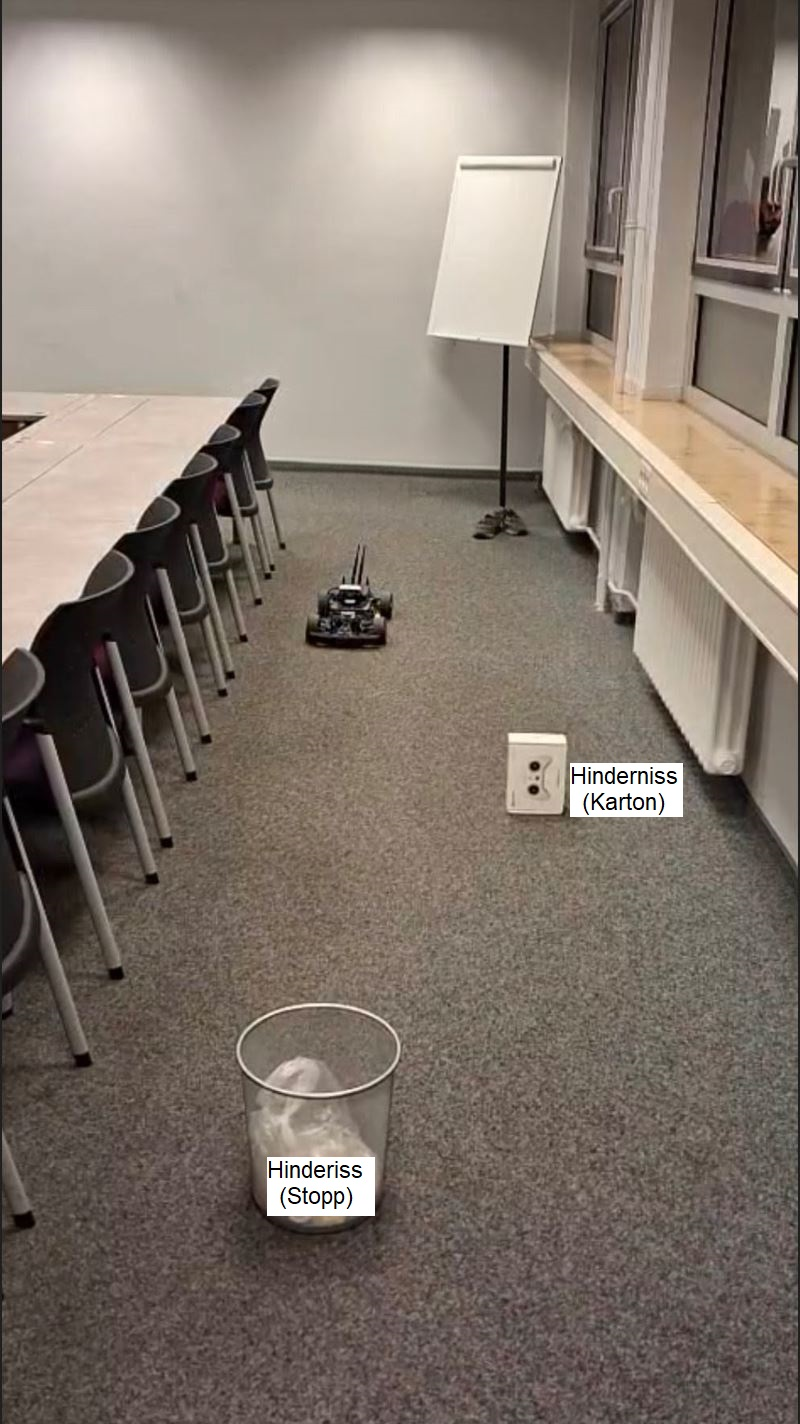
\includegraphics[width=0.95\textwidth]{images/foxglove_validation_overview.png}
    \caption{Exemplarisches Foxglove-Layout zur Online-Beobachtung des FTG-Stacks während der Validierungsfahrten. Dargestellt sind Sensorik, Visualisierungstopics und zentrale Zustandsgrößen des Planungs- und Steuerpfads.}
    \label{fig:foxglove_validation}
\end{figure}

Die eigentliche quantitative Bewertung erfolgte auf Basis der aufgezeichneten Bags in einer
anschließenden Offline-Analyse. Hierzu wurden die Signalverläufe der beiden Validierungsläufe
zeitlich ausgewertet und in Form von Metriken und Zeitreihenplots aufbereitet. Zu den
wesentlichen Kenngrößen zählen unter anderem:

\begin{itemize}
    \item mittlerer und minimaler Frontabstand,
    \item mittlere Sollgeschwindigkeit und Zeitanteil mit Stopp-Anforderung,
    \item Zeitanteil mit erfolgreicher Gap-Erkennung,
    \item Auftreten von Sättigungen im Heading- bzw. Gap-Winkel,
    \item Auftreten von Planner-Zuständen wie \textit{normal}, \textit{stale} oder \textit{no valid gap found}.
\end{itemize}

Die daraus resultierenden Validierungsplots und metrischen Vergleiche werden in Kapitel~\ref{ch:diskussion}
zur Diskussion und Bewertung der beiden Teststrecken herangezogen.
